%=================================================================

\section{Introduction}\label{sec-intro}

\subsection{Problem Statement}
\

After a month of making scientific observations 
and taking careful measurements, 
can determined that 900 ghouls, ghosts, and goblins
like what is shown in~\Cref{fig:animal}  .
The raw dataset contains train set with 371 
samples and 529 unlabeled samples as test set.
Through the train data, find the relationship
between the attributes and species, 
and then identify 371 of the ghastly creatures.


\begin{figure}[htbp]
	\centering
	%\graphicspath{figures}
	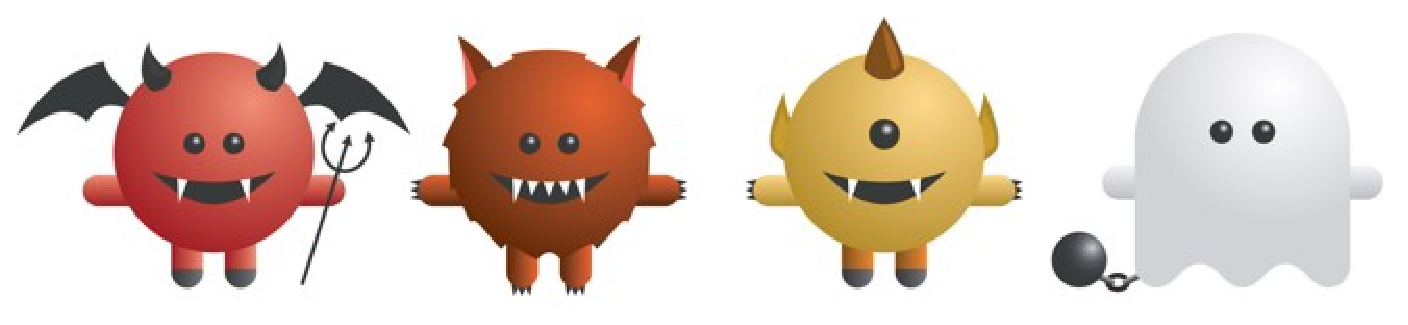
\includegraphics[scale=0.3]{figures/bar.eps}
	\caption{The Picture of Ghastly}\label{fig:animal}
\end{figure}


\subsection{Data List}
\

There are bone length measurements, 
severity of rot, extent of soullessness, 
and other characteristics of the intruders,
the fllowings are the  
name and meaning of attributes


\begin{description}
	\item[id] id of the creature
	\item[bone\_length] average length of bone in the creature, normalized between 0 and 1
	\item[rotting\_flesh] percentage of rotting flesh in the creature
	\item[hair\_length] average hair length, normalized between 0 and 1
	\item[has\_soul] percentage of soul in the creature
	\item[Color] dominant color of the creature: 'white','black','clear','blue','green','blood'
	\item[type] target variable: 'Ghost', 'Goblin', and 'Ghoul'
\end{description}


\subsection{Problem Analysis}

\subsubsection{Train Data and Test Data}
\

Because this game is over, 
it can't submit the predictive values for testing. 
So I divide the raw train data into train data and test data, 
and the ratio is 8:2. 
Another vexed problem is the data too small, 
so I use ten-fold cross-validation 
to train the models.


\subsubsection{Problem Possible Solutions}
\

There are many machine learning algorithms 
can solve the three classification problem,
such as ensemble algorithms,
decision tree algorithm and so on.
Use CV to find the best parameters of the algorithms 
and then validate with testing data.
But the most important thing is 
do  feature engineering to improve accuracy. 


\subsubsection{Evaluation Methods}


Before experiment, determine the evaluation methods
to assess the model performance is very important,
usually it has the following methods
for classification problem:

\begin{itemize}
	\item F1 Score/AUC
	\item Class Accuracy
\end{itemize} 


\section{Data exploration} \label{sec-data_exploration}

\subsection{Data Information}
\

The following  ~\cref{tbl:data information}
is the statistical result of the attribute values.
There are 4 numerical variables and 1 categorical,
and no missing values.
Numerical columns are either normalized or show a percentage, 
so no need to scale them. 

\begin{table}[htbp]  \centering
	\caption{Data Information}
	\label{tbl:data information}
	\begin{tabular}{ccccccc}
		\hline
		% after \\: \hline or \cline{col1-col2} \cline{col3-col4} ...
		& bone\_length & rotting\_flesh & hair\_length & has\_soul & color & type\\
		\hline
		count & 371.0 & 371.0 & 371.0 & 371.0 & 371 & 371 \\
		unique & NaN & NaN & NaN & NaN & 6 & 3 \\
		top & NaN & NaN & NaN & NaN & white & Ghoul \\
		freq & NaN & NaN & NaN & NaN & 137 & 129\\
		mean & 0.434160 & 0.506848 & 0.529114 & 0.471392 & NaN & NaN \\
		std & 0.132833 & 0.146358 & 0.169902 & 0.176129 & NaN & NaN \\
		min & 0.061032 & 0.095687 & 0.134600 & 0.009402 & NaN & NaN \\
		25\% & 0.340006 & 0.414812 & 0.407428 & 0.348002 & NaN & NaN \\
		50\% & 0.43891 & 0.501552 & 0.538642 & 0.466372 & NaN & NaN\\
		75\% & 0.517223 & 0.603977 & 0.647244 & 0.600610 & NaN & NaN\\
		max &  0.817001 & 0.932466 & 1.000000 & 0.935721 & NaN & NaN\\
		\hline 
		%\bottomrule
	\end{tabular}
\end{table}


\subsection{Data Visualization}
\

Use EDA to plot the distribution of the data,
can observate the data intuitively and
find the relation between the attribute values. 
For example boxplot can visually observe 
the distribution of numerical variables, 
scatterplot can show their distribution trends 
and whether exists outliers.
For classification problems, 
the data with the same label is drawn in same color, 
which is very helpful for 
the construction of the Feature.


\subsubsection{ Histogram}
\

The figure ~\Cref{fig:his_1} 
shows the mean of the four numerical variables  
and the figure ~\Cref{fig:his_2} 
is the number of different color 
about types of ghastly creatures.
It seems that all numerical features may be useful, 
but many colors are evenly distributes among the monsters,
which means they maybe have little effect on classification.


\begin{figure}[htbp]
	\centering
	
	%\graphicspath{{figures/}{mine/}}
	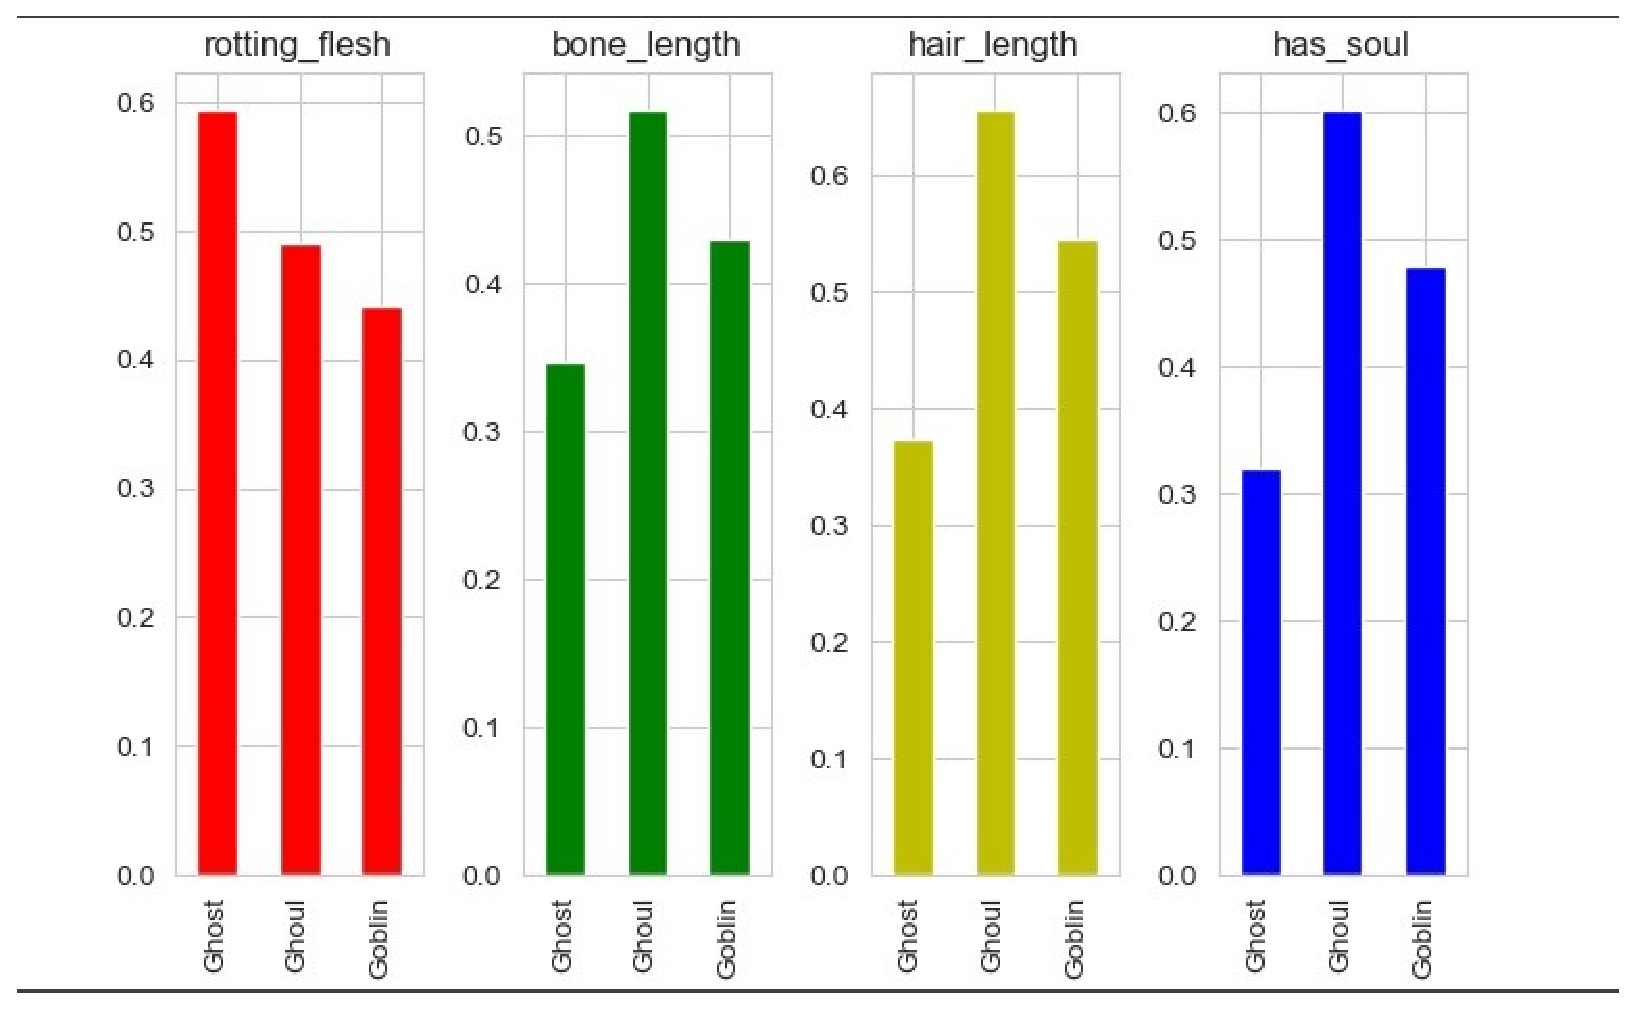
\includegraphics[scale=0.3]{figures/his_1.eps}
	\caption{The Mean of Four Numerical Variables}\label{fig:his_1}
\end{figure}

\begin{figure}[htbp]
	\centering
	
	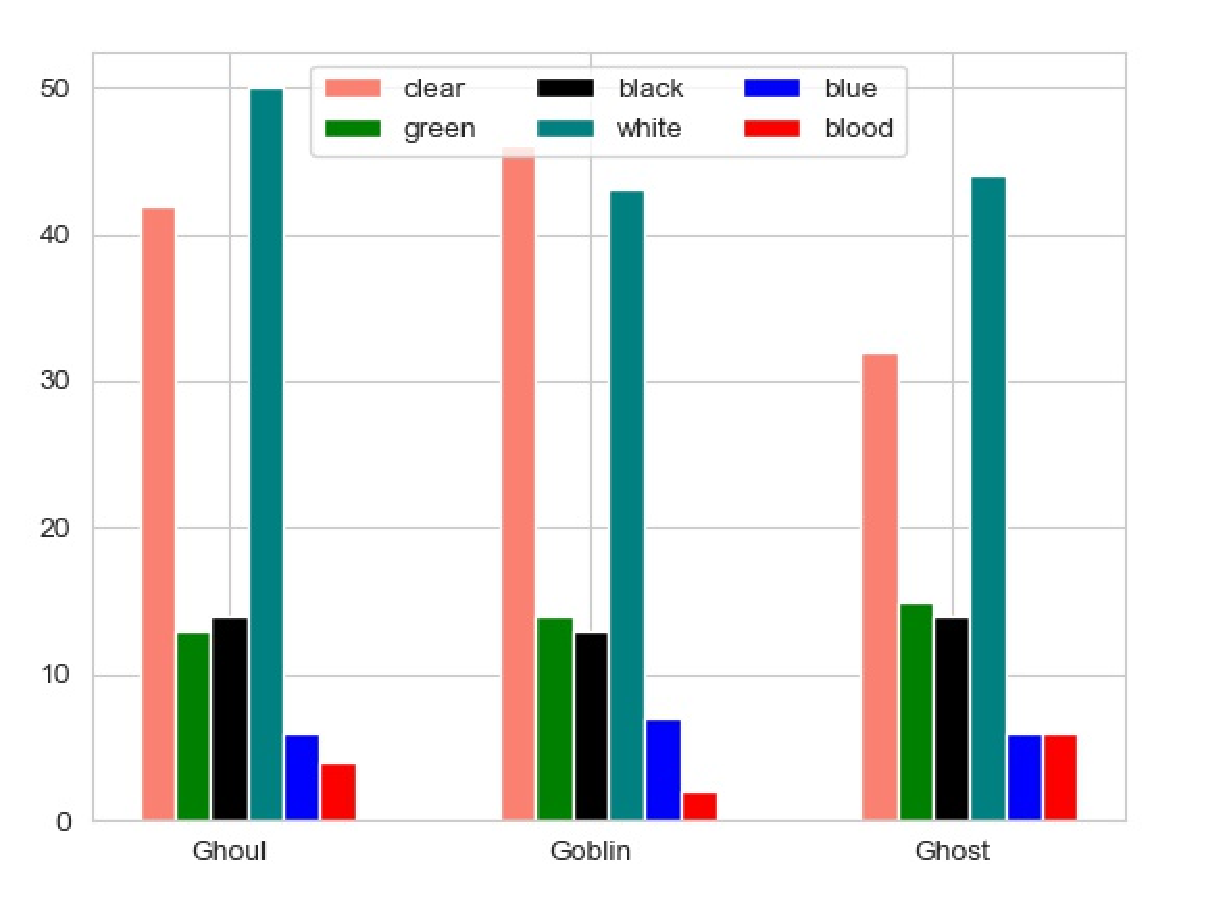
\includegraphics[scale=0.3]{figures/his_2.eps}
	\caption{Color distribution Grouped by Type}\label{fig:his_2}
\end{figure}

\subsubsection{Boxplot}
\
 
When analyzing the data, 
the boxplot can effectively 
help us identify the characteristics of the data:
visually identify outliers in the dataset or
determine the data dispersion and 
bias of the data set. 
Through the figure ~\Cref{fig:boxplot}, 
we know that the two types of Ghost and Ghoul 
in the monster have higher discrimination 
on the four variables, 
while Goblin is in the middle position, 
which intersects with the other two types of features.
Based on the above observation,
we guess that the predictive accuracy of Ghost and Ghoul 
will be better than Goblin.
And the outliers are very small,
which can be ignored.


\begin{figure}[htbp]
	\centering
	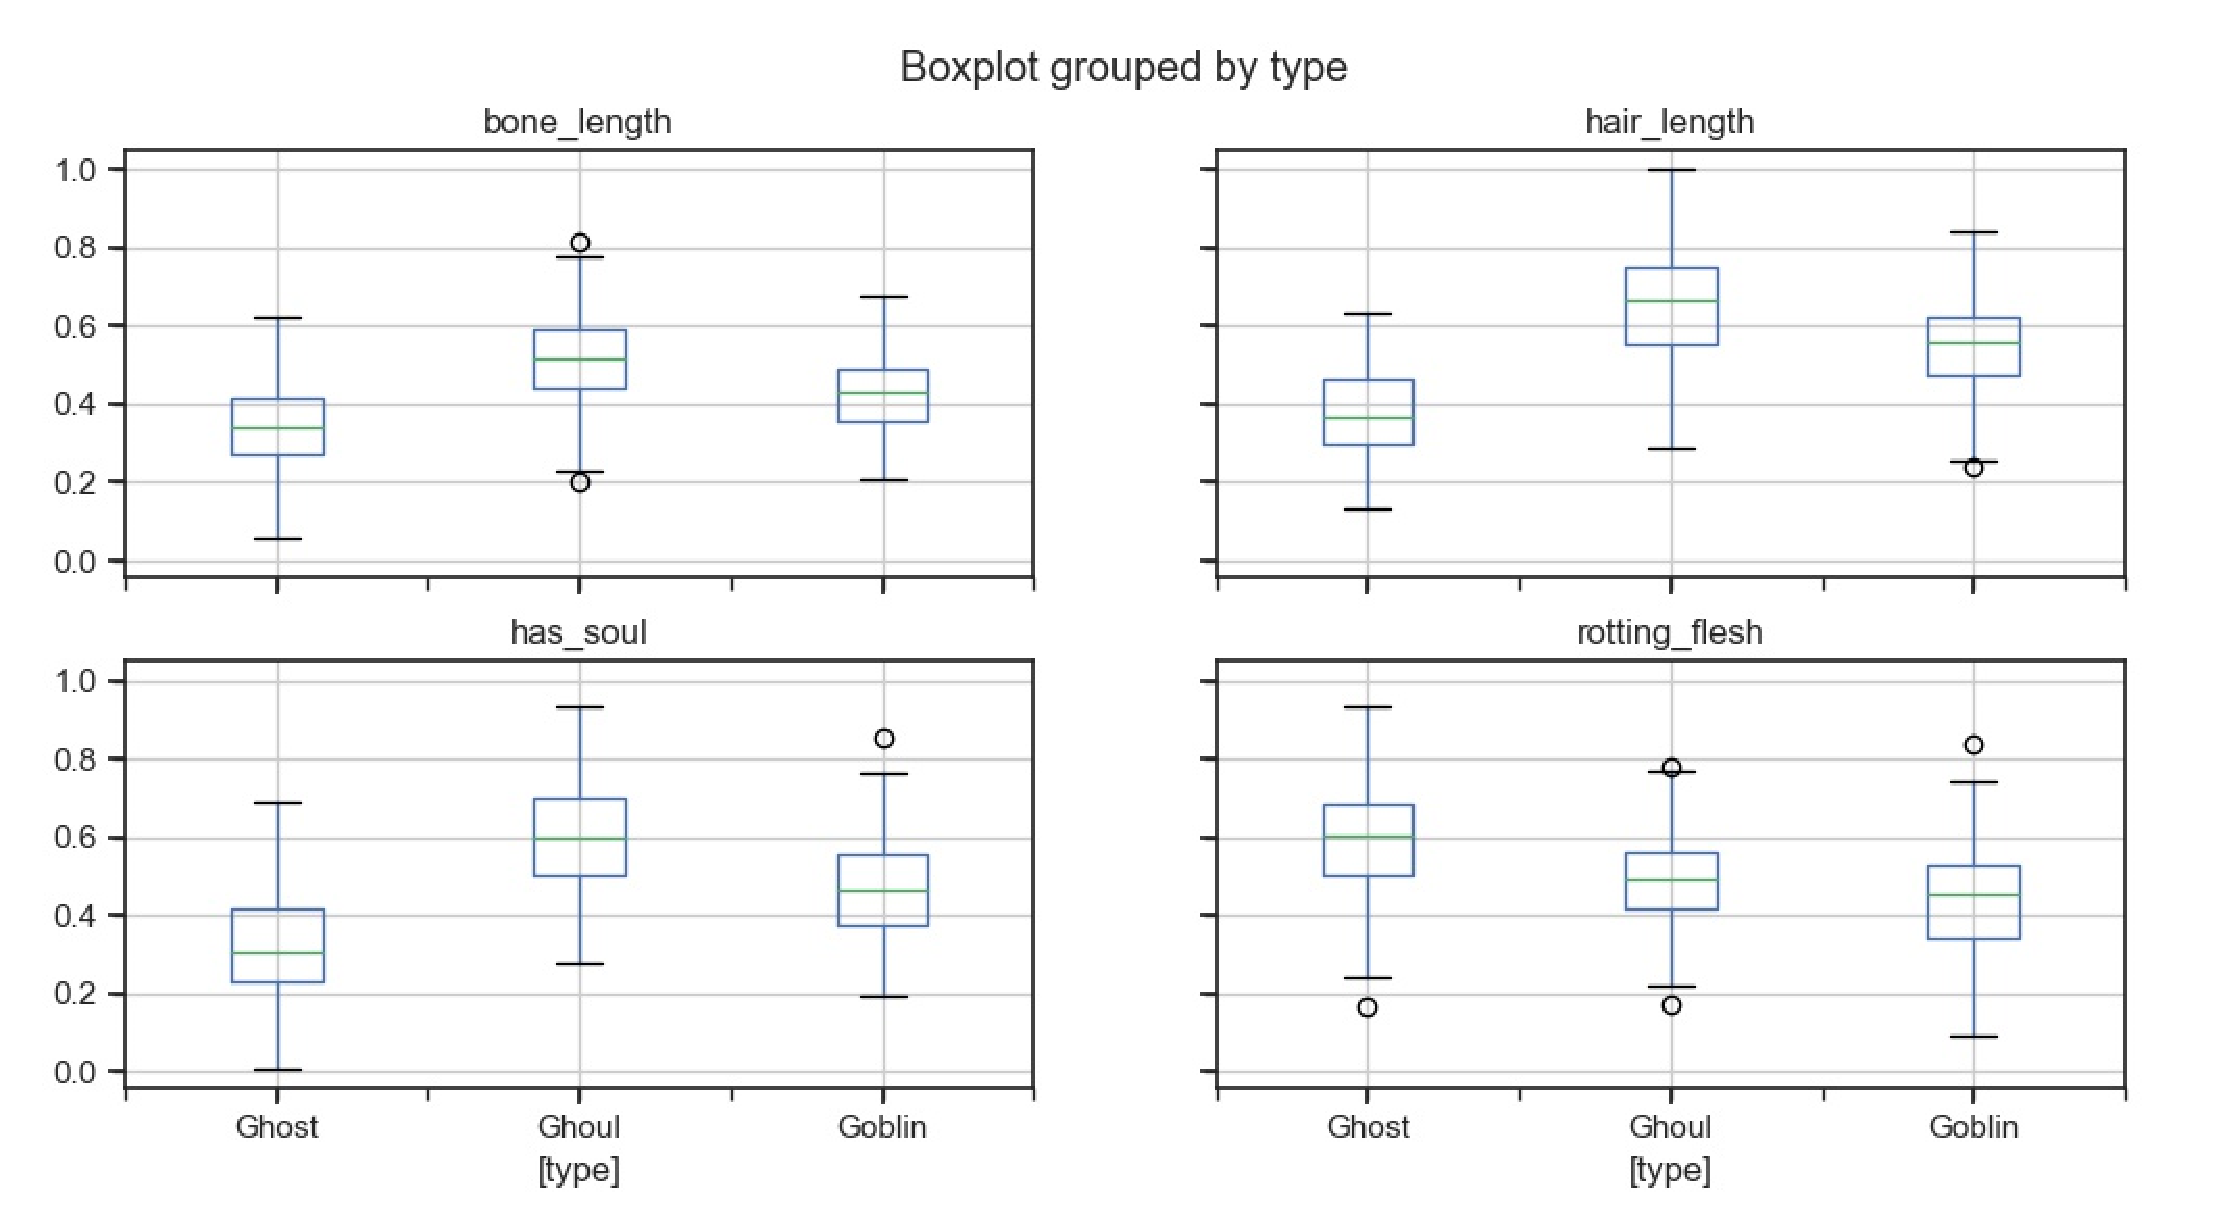
\includegraphics[scale=0.3]{figures/boxplot.eps}
	\caption{Boxplot Grouped by Type}\label{fig:boxplot}
\end{figure}


\subsubsection{Pairwise Plot} 
\

Pairwise plot is 
a favorite in exploratory analysis 
to understand the relationship 
between all possible pairs 
of numeric variables. 
This pairplot ~\Cref{fig:feature_scatterplot} 
shows that data is distributed normally. 
And while most pairs are widely scattered 
(in relationship to the type), 
some of them show clusters: 
hair\_length and has\_soul, 
hair\_length and bone\_length. 
So it may need to reassemble the data.

\begin{figure}[htbp]
	\centering
	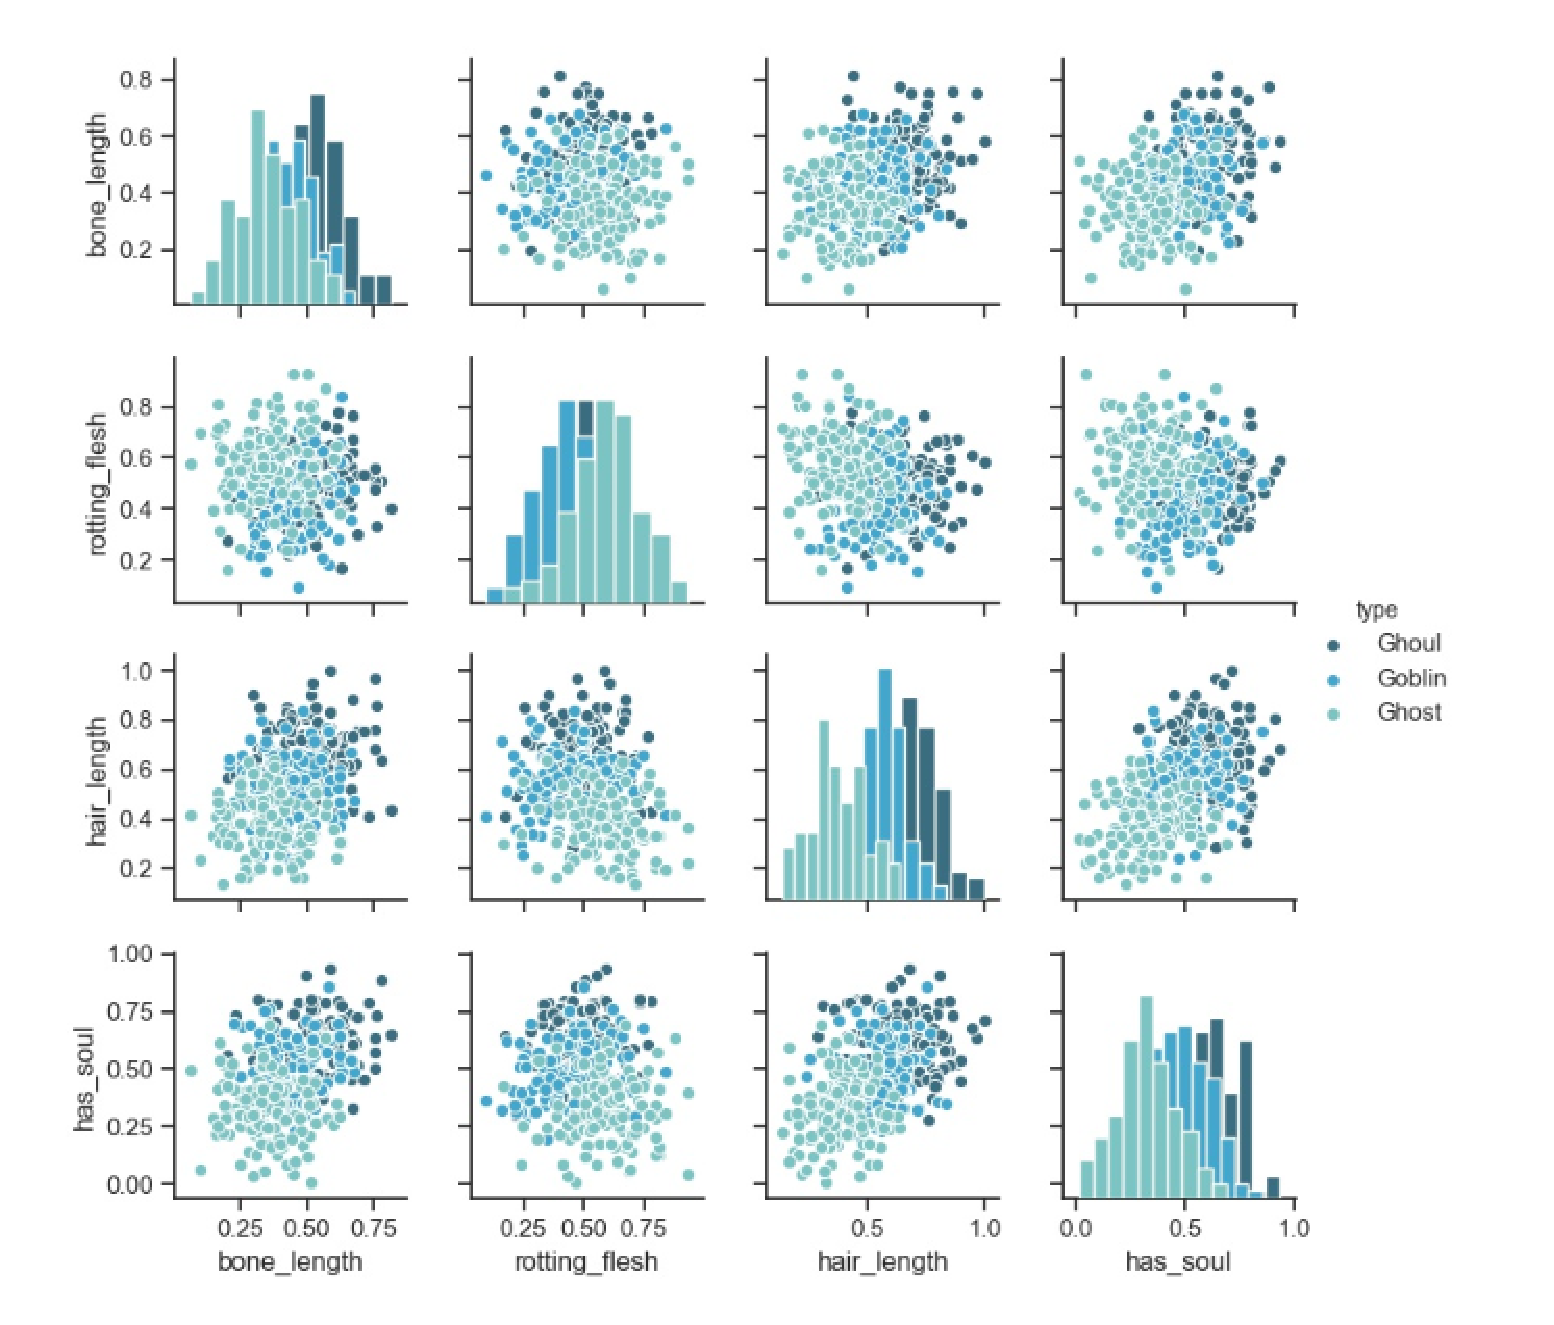
\includegraphics[scale=0.4]{figures/pairplot.eps}
	\caption{Feature Scatterplot}\label{fig:feature_scatterplot}
\end{figure}

\subsubsection{Correllogram}
\

Correlogram is used to 
visually see the correlation metric 
between all possible pairs of numeric variables 
in a given dataframe. 
This figure ~\Cref{fig:corr} 
make it convenient for us to analyze features,
especially their impact on the 'type' column. 
As we can see the 'type' column 
has a high value of negative correlation 
with columns 'has\_soul' and 'rotting\_flesh',
but the correlation 
with the 'hair\_length' is not very big.
There is no obvious linear relationship 
between these variables.

\begin{figure}[htbp]
	\centering
	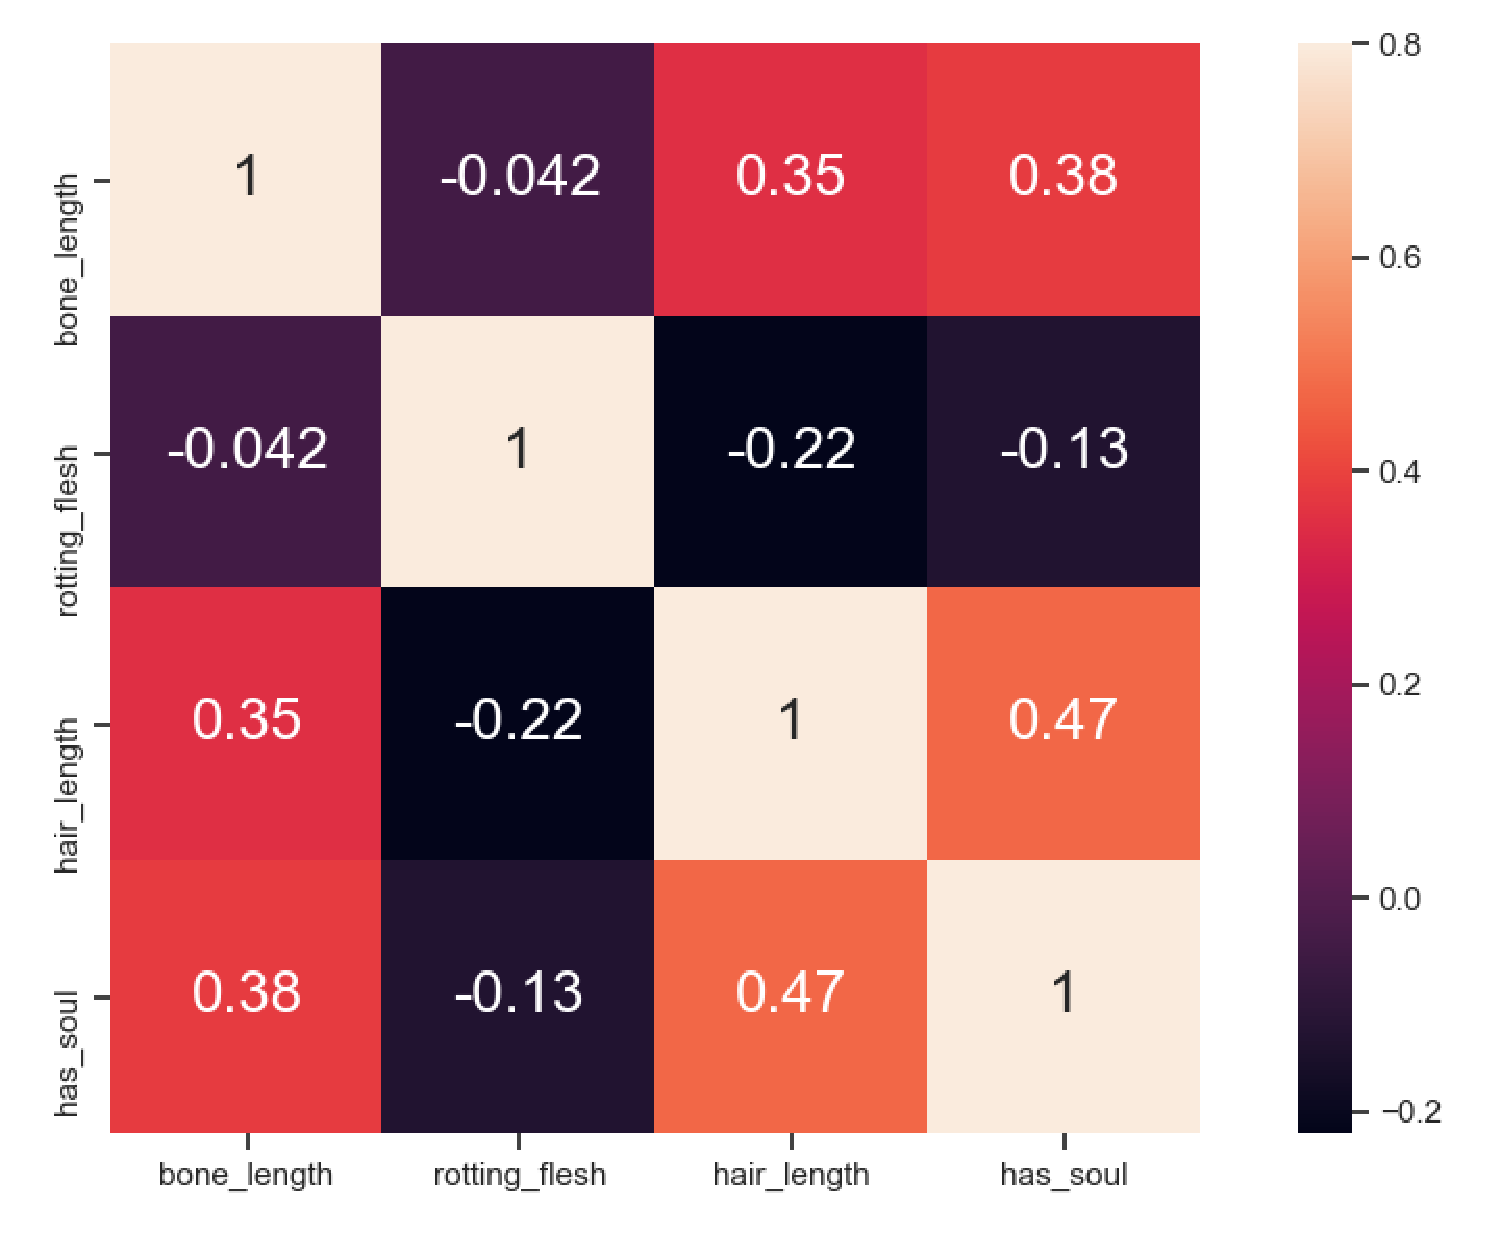
\includegraphics[scale=0.4]{figures/corr.eps}
	\caption{Correllogram}\label{fig:corr}
\end{figure}


\subsubsection{Other Figures}


The following pictures 
are independent of 
the choice of algorithm,
Because they look great, 
so I want to share with you.
%如果有时间的话,把这三张图片放在一排,然后稍微介绍一下

\begin{figure}[h]\centering
	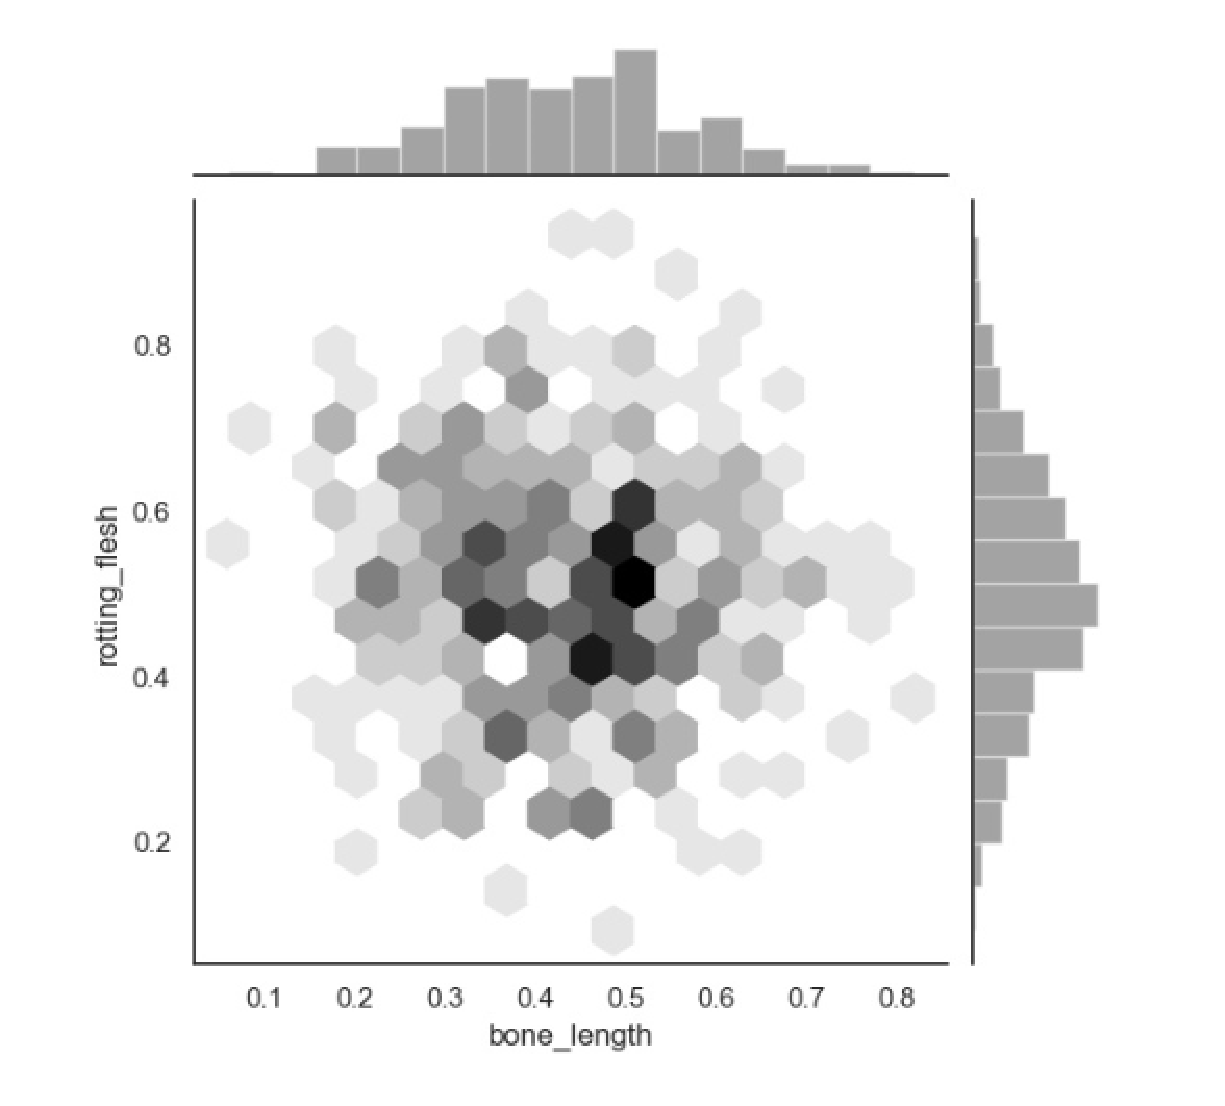
\includegraphics[scale=0.4]{figures/MHis.eps}
	\caption{Marginal Histogram}
\end{figure}

\begin{figure}[h]\centering
	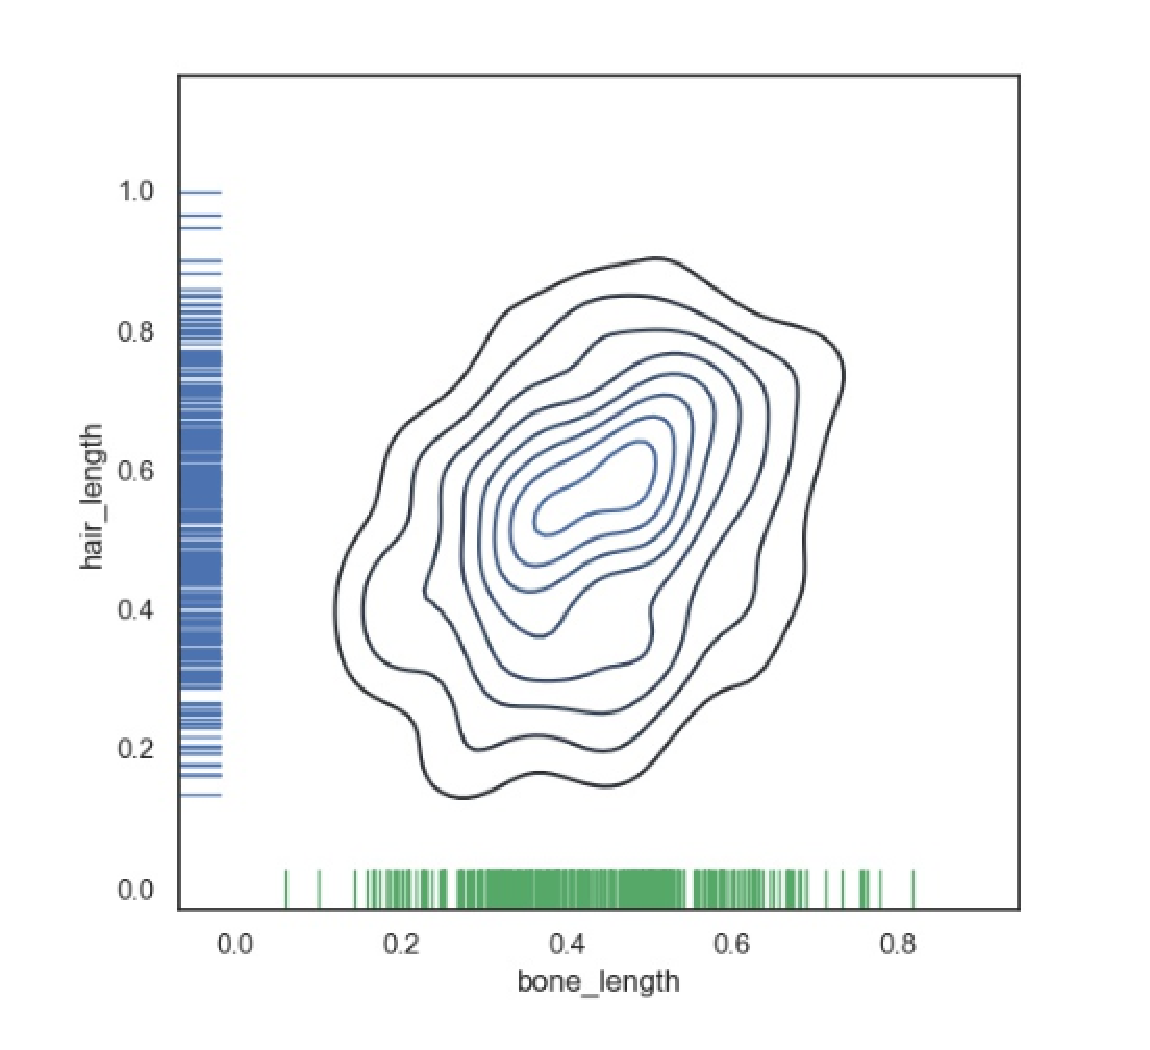
\includegraphics[scale=0.4]{figures/BDF.eps}
	\caption{Binary Density Function}
\end{figure}

\begin{figure}[h]\centering
	%\graphicspath{{figures/}{mine/}}
	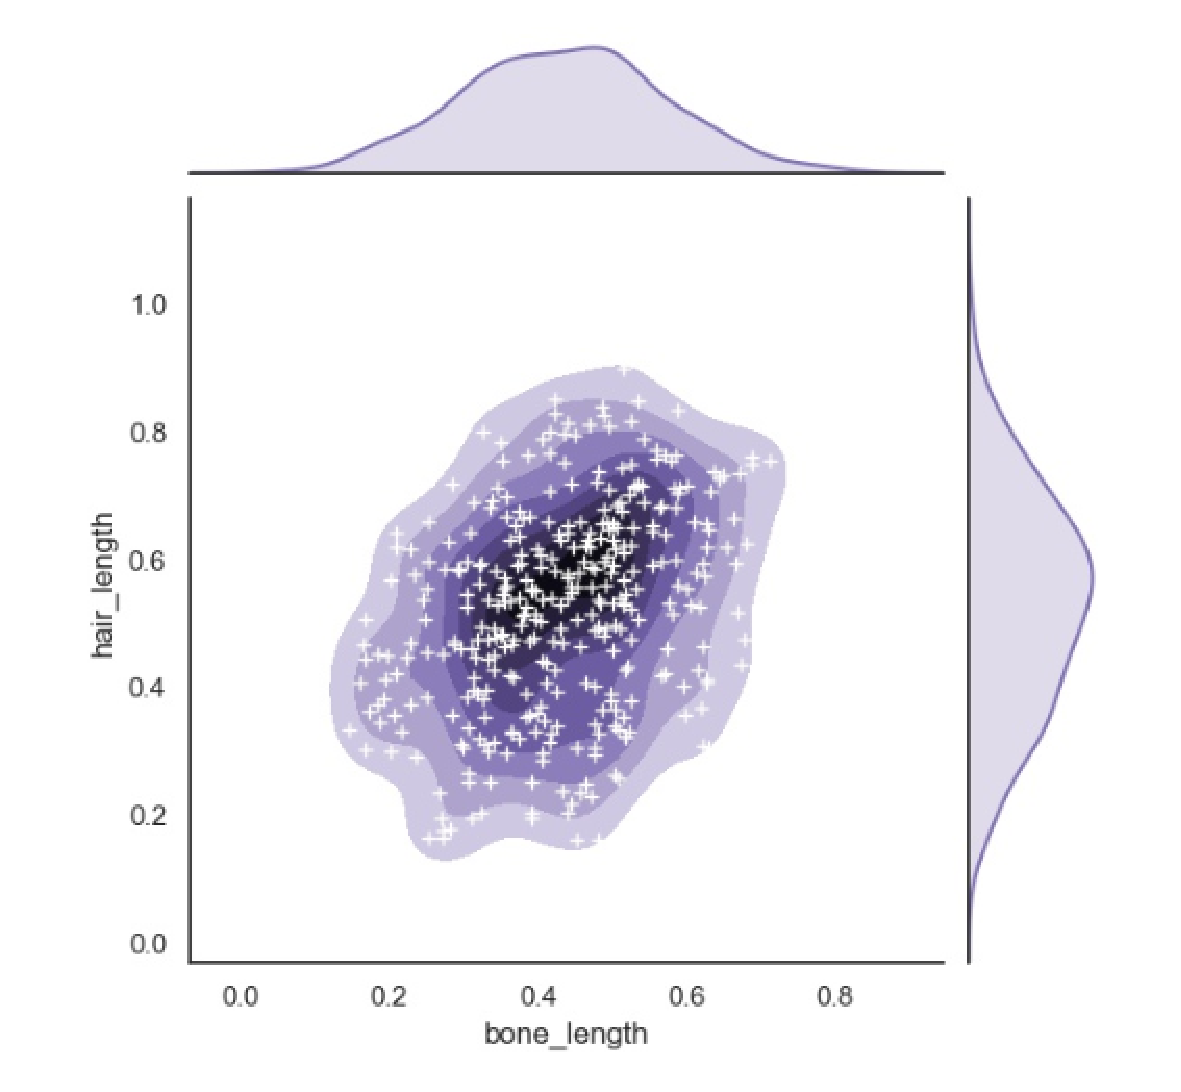
\includegraphics[scale=0.4]{figures/MBDF.eps}
	\caption{Marginal Binary Density Function}
\end{figure}


\subsection{Data Preparation}

\subsubsection{Great New Features}
\

As it can be seen from 
the pictures above 
the data is distributed normally. 
But some of them show clusters: 
hair\_length and has\_soul, 
hair\_length and bone\_length. 
So I create new variables 
with multiplication of these columns: 

\begin{description}
	\item[hair\_soul] row[hair\_length]*row[has\_soul] 
	\item[hair\_bone]  row[hair\_length]*row[bone\_length] 
	\item[bone\_soul]  row[bone\_length]*row[has\_soul] 
	\item[hair\_soul\_bone]  row[hair\_length]*row[has\_soul]*row[bone\_length] 
\end{description}


Then analyse the new features in a pairplot, 
showing the picture ~\Cref{fig:new_pairplot}
below. 
It can be seen from the picture that 
there is a clear linear relationship 
between the variables. 


\begin{figure}[htbp]
	\centering
	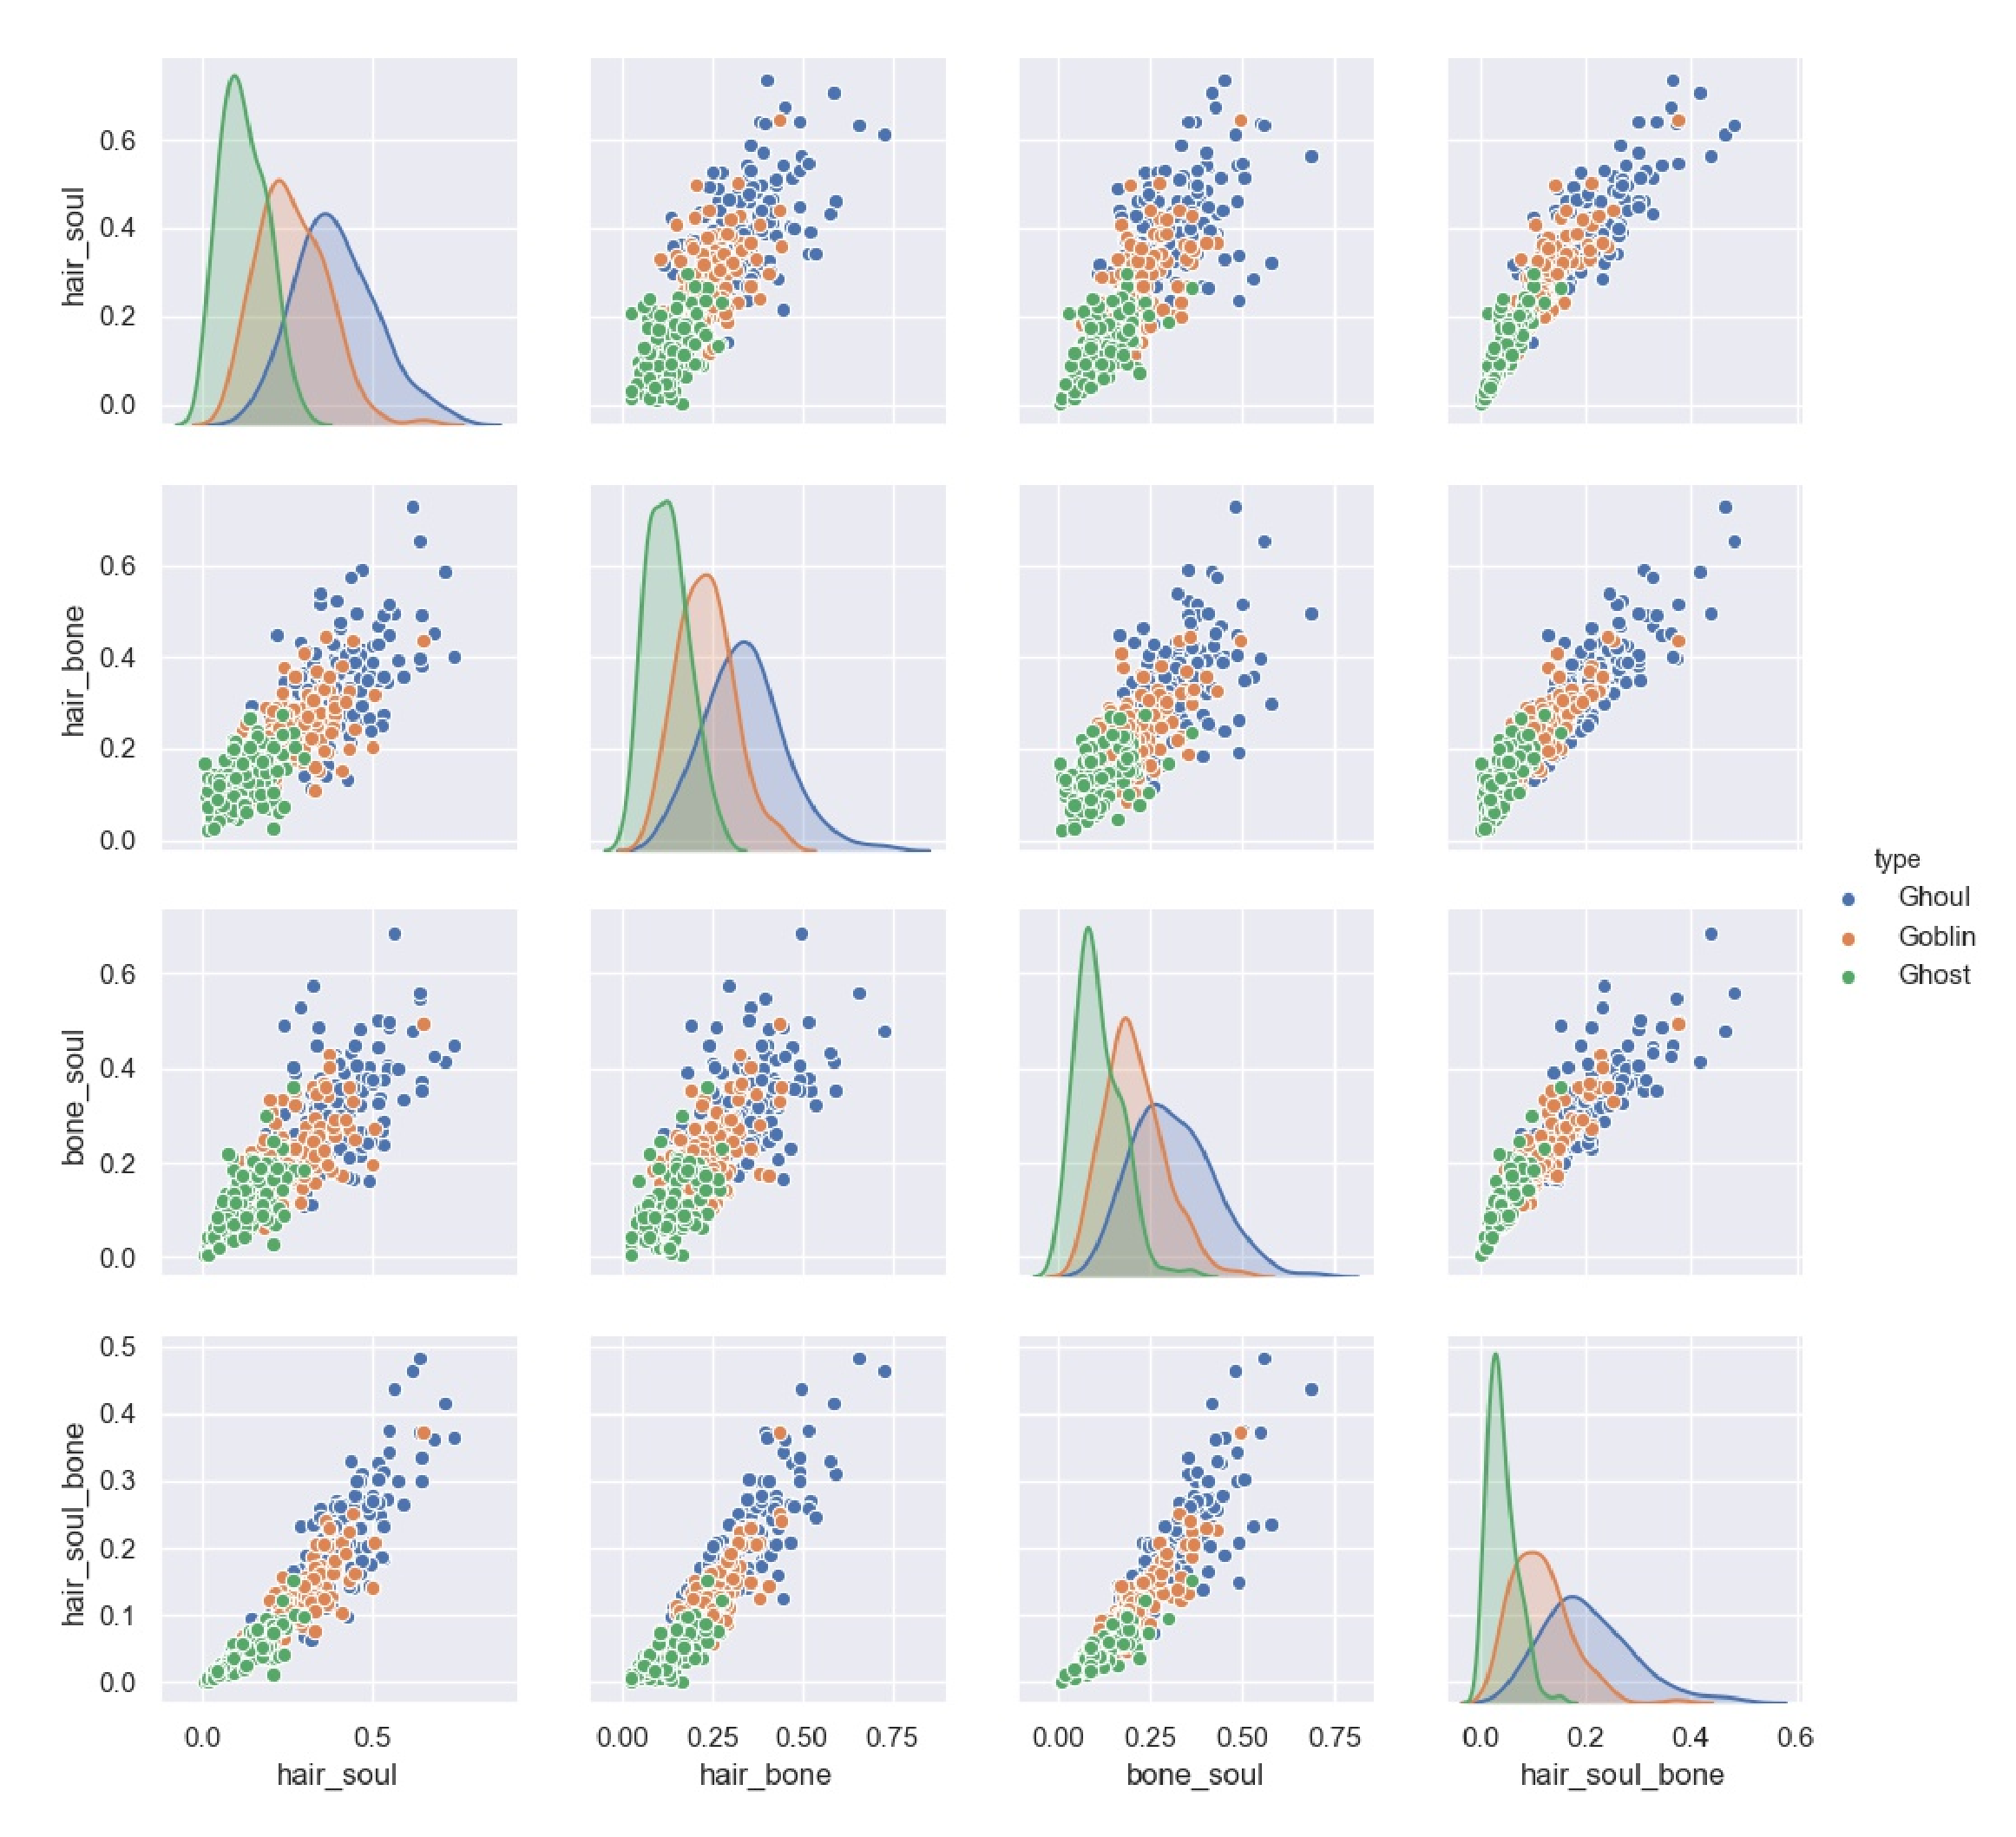
\includegraphics[scale=0.3]{figures/hist_1.eps}
	\caption{New Features Pairplot}\label{fig:new_pairplot}
\end{figure}


\subsubsection{Feature Selection}
\

Use the algorithm below to 
calculate the importance of features.
The following figure ~\Cref{fig:feature_importance}
is a histogram ordered by feature importance. 

\begin{algorithm}[htbp]
	\small
	\caption{Features Selection}
	\label{alg:features_selection}
	\begin{algorithmic}[1]
		\REQUIRE
		Features $X=\{ X_1, X_2, ... , X_n \}$,
		The number of tree node $M$,
		$GI_m$ Gini index of node $m$, 
		$ K $ the number of target,
		$ p_mk $ proportion of target $k$ in node $m$,
		$ VIM_{jm}^{\small(Gini)} $ the importance of feature $X_j$ in node $m$ ,
		$ n$ the tree number of RF.
		\ENSURE
		Variable Importance Measures $VIM_{j}^{\small(Gini)}$.
		\STATE
		Initialize $GI_m$ , 
		$VIM_{j}^{\small(Gini)} $;
		\FOR {$m \leftarrow 1...M$}
		\FOR {$k \leftarrow 1...K$}
		\STATE Compute the Gini index of node $m$
		$GI_m = \sum_{k=1}^{|K|} \sum_{k'\neq k} {p_{mk}}{p_{mk'}}=1- \sum_{k=1}^{|K|} p^2_{mk}$
		\ENDFOR
		\STATE Divide node m into node r and node l
		\STATE Compute the importance of feature $X_j$ in node $m$ 
		$VIM_{jm}^{\small(Gini)} = GI_m-GI_l-GI_r $
		\ENDFOR
		\FOR {$i \leftarrow 1...N$}
		\STATE Compute variable importance measures 
		$VIM_{j}^{\small(Gini)} = VIM_{j}^{\small(Gini)} + VIM_{ij}^{\small(Gini)}$
		\ENDFOR
		\RETURN $VIM_{j}^{\small(Gini)}$
	\end{algorithmic}
    %\caption{Feature Selection Algorithm}
\end{algorithm}

\begin{figure}[htbp]
	\centering
	%\graphicspath{{figures/}{mine/}}
	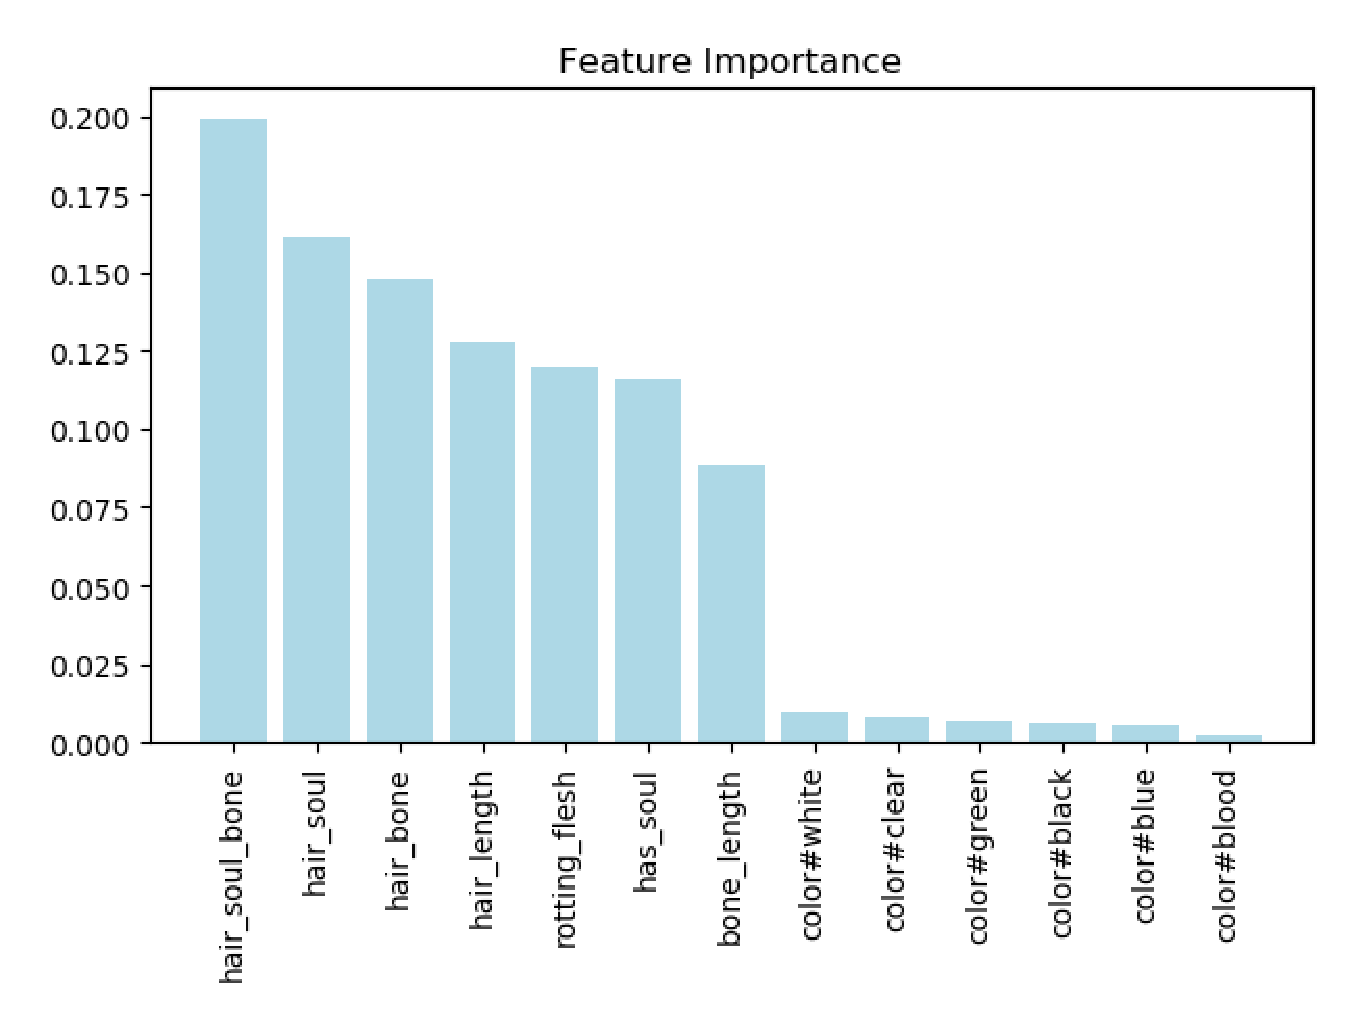
\includegraphics[scale=0.3]{figures/FEATURE.eps}
	\caption{Feature Importance}\label{fig:feature_importance}
\end{figure}

We take the top seven features 
with higher importance 
to form a new train data, the rest are discarded.


\section{Methods}

There are many machine learning algorithms 
for classification problem. 
Choose the following algorithms, 
explain the principles of
these algorithms and 
show the most important parameters.

\begin{itemize}
	\item RandomForest 
	\item Bagging
	\item GradientBoosting
	\item LogisticRegression
	\item SVC
	\item KNeighbors 
	\item XGBoost
	\item Netual Network
\end{itemize}

\subsection{RandomForest}
\

Random forest is a classifier with 
multiple decision trees, and
the output is determined by 
the mode of the individual tree output.

\begin{itemize}
	\item Principle
	
	\begin{itemize}
		\item Use M to indicate the number of training samples, 
		and N to indicate the number of features.
		\item The number of feature inputs n is 
		used to determine the decision result 
		of a node on the decision tree; 
		where n should be much smaller than N.
		\item From the M training samples, 
		the sampling is performed k times to 
		form a training set (ie bootstrap sampling), 
		and the unused use cases (samples) are 
		used for prediction to evaluate the error.
		\item For each node, 
		n features are randomly selected, 
		and the decision of each node on each decision tree is 
		determined based on these characteristics. 
		According to these n features, 
		calculate the best split mode.
		\item Finally, predict the test data and 
		decide the classification 
		according to each tree in a multi-winning manner.
	\end{itemize}
	
	\item Parameters
	
	\begin{description}
		\item[n_estimators] the number of decision trees
		\item[criteriom] criterion of choosing 
		the most appropriate node
		\item[max_depth] The maximum depth of the tree, 
		the default is None 
		\item[max_features] The feature that is divided 
		when selecting the optimal attribute 
		cannot exceed this value.
	\end{description}

\end{itemize}


\subsection{LogisticRegression}
\

Logistic regression is the algorithm that 
processing a large amount of 
observation data to 
obtain mathematical expressions 
that are in line with 
the internal laws of things

\begin{itemize}
	\item Principle
	
	\begin{description}
		\item[Hypothesis] $h(x)=W^{T} x+b$
		\item[Parameters] $ W$, $x$
	\end{description}
	
	\item Parameters
	
	\begin{description}
		\item[Penalty] Regular function
		\item[C] Regular coefficient
	\end{description}
	
\end{itemize}
%J=sum(logloss(f(xi), yi)) + C* penalty

\subsection{Bagging}
\

Bagging can improve the stability and accuracy 
of machine learning algorithms, 
it can reduce the variance of 
the model and avoid overfitting

\begin{itemize}
	\item Principle
	
	\begin{description}
		\item[INPUT] train data $ D = \left\{ 
		\left(x_1,y_1 \right), \left(x_2,y_2 \right),
		\dots,\left(x_m,y_m \right) \right\}$
		
		Base learning algorithm $L$
	
		Frequency of training $T$
		\item[OUTPUT] The best base learning algorithm $f(x)$
	
	\end{description}
	
	\item Parameters
	
	\begin{description}
		\item[n_estimators] Number of combined basic evaluators
		\item[max_samples] Number of basic estimator samples
	\end{description}
	
\end{itemize}

\subsection{GradientBoosting}
\

Gradient boosting uses gradient descend 
to find the best solvtion.
A major step in machine learning is 
to minimize the loss function $L(θ)$ 
by an optimization method to 
find the corresponding parameter $θ$. 
Gradient descent is 
a classic numerical optimization method.

\begin{itemize}
	\item Principle
	
	\begin{description}
		\item[Initialization] $ f_{0}(x)=	
		\operatorname{arg\,max}_\gamma 
		\sum\nolimits_{i=1}^n L(y_i,\gamma)$
		
		\item[for $m=1$ to $M$] 
		\
		
		\begin{itemize}
			\item calculate negative gradient
			\item through minimizing the square error, 
			fitting the $ \tilde{y_i} $ 
			with the base learner $h_m(x)$
			\item use line search to 
			determine the step size $\rho_m$ to minimize $L$
		\end{itemize}
		
		\item[OUTPUT] $f_M(x)$
	\end{description}
	
	\item Parameters
	
	\begin{description}
		\item[learning_rate] control the speed of each update
		\item[n_estimators] he number of decision trees that 
		need to be used
		\item[max_depth] the maximum depth of the tree
	\end{description}
\end{itemize}
%\frac{\partial f}{\partial x} = 2\,\sqrt{a}\,x
\subsection{SVC}
\

The basic principle of the SVM algorithm is 
to find a hyper plane that can 
distinguish between two types, 
so that the margin is the largest.

\begin{itemize}
	\item Princible
	
	\begin{itemize}
		\item choose a kernel function, reduce the amount of calculation
		\item determining the hyperplane equation
		\item optimization model
	\end{itemize}

	\item Parameters
	
	\begin{description}
		\item[kernel] kernel function
		\item[C] penalty factor for error terms
		\item[degree] order of polynomial kernel function
	\end{description}
	
\end{itemize}

\subsection{KNeighbors}
\

The meaning of the knn algorithm is that 
enter new data without tags, 
compare each feature of the new data with 
each feature in the training set, 
and select the classification tag with 
the most similar feature (nearest neighbor: k)

\begin{itemize}
	\item Princible
	\begin{itemize}
		\item calculate the Euler distance of 
		the new sample point in the sample space 
		from all training samples
		\item Sort the Euler distances and 
		find the nearest k points
		\item Classify statistics on k points to 
		see which type of points has 
		the most number. 
		This type is the type of 
		prediction for new samples.
	\end{itemize}
	
	\item Parameters
	\begin{description}
		\item[n_neighbors] number of neighbors to use 
		by default for kneighbors queries
		\item[leaf_size] leaf size passed to BallTree or KDTree
		\item[p] power parameter for choosing 
		the distance calculation formula
		\item[weights] used in prediction
		\item[algorithm] compute the nearest neighbors
	\end{description}
	
\end{itemize}

\subsection{XGBoost}
\
 
XGBoost is to establish K regression trees 
so that the predicted value of 
the tree group is as close as possible to 
the true value (accuracy) and 
has the greatest generalization ability. 
From a mathematical point of view, 
this is a functional optimization, multi-target.

\begin{itemize}
	\item Princible
	\begin{description}
		\item[predictive model] $\hat{y_i}=\sum\nolimits_{k=1}^K f_k(x_i)$
		
		$K$ is the number of trees,
		$f_k$ represents the kth tree,
		$\hat{y_i}$ is the predictive result of $x_i$
		\item[loss function] $Obj(\theta)=\sum\nolimits_{i=1}^n l(y_i,\hat{y_i})+
		\sum\nolimits_{k=1}^K \Omega(f_k)$
		
		$l(y_i,\hat{y_i}$ is the train error of example 
		$x-i$, $\Omega(f_k)$ is the regular item of the kth tree.
	\end{description}
	
	\item Parameters
	\begin{description}
		\item[learning_rate]  control the speed of each update
		\item[n_estimators] number of iterations
		\item[max_depth] the depth of tree
		\item[gamma] penalty factor%惩罚系数
		\item[subsample] the proportion of data used in 
		all training sets when training each tree
		\item[colsample_bytree] the proportion of features used 
		in all trees when training each tree
	\end{description}
\end{itemize} 

\subsection{Netual Network}
\

Netual network is widely used in various fields.

\begin{itemize}
	\item Princible
	
	The neural network generally consists of 
	an Input Layer, a Hidden Layer, and an Output Layer. 
	Each layer is composed of Units. 
	The input layer is passed in by 
	the instance feature vector of the training set. 
	The weight of the node is passed to the next layer. 
	The output of the upper layer is 
	the input of the next layer. 
	The number of hidden layers is arbitrary. 
	There is only one output layer and input layer.
	
	\item Parameters
	
	\begin{description}
		\item[hidden_layer_sizes] The i-th element represents 
		the number of neurons in the i-th hidden layer
		\item[activation] activation function
		\item[solver] weight optimization solver
		\item[learning_rate] weight update speed
	\end{description}
\end{itemize}

\subsection{Ensemble Model}
\

There are many machine learning algorithms, 
use the above machine learning algorithms 
as Ensemble Model’s base models. 
Through Grid Search and
ten-fold cross-validation
to find the optimal parameters.

\section{Experiment and Analysis}

In the Data Exploration, 
I has created some new feaures.
The following experiment is divided into two parts,
one is to use the original train data, 
the other is to use new features as train data.
Grid Search make it easier to 
determine a set of optimal parameters
for these model I adpot.
Because the train data is relatively small, 
a ten-fold cross-validation is used. 
Then I can test the trained models 
using test data and 
analyze the experimental results.
And use the trained models as 
the base models of ensemble model,
then do experiment. 
\WBJianginMarker

\subsection{Base Models Training Result}
\subsubsection{Original Train Data}
\

The following are the best parameters and 
the Best Score in training of 
the base models 
in original train data. 

\begin{itemize}
	\item Best Parameters of Models
	\begin{description}
		\item[RandomForest] 'criterion': 'entropy', 'max_depth': 5, 
		'max_features': None, 'n_estimators': 100
		\item[Bagging] 'max_samples': 10, 'n_estimators': 100,
		'n_estimators': 100
		\item[GradientBoosting] 'learning_rate': 0.3, 'max_depth': 2, 
		'n_estimators': 20
		\item[LogisticRegression] 'C': 1, 'penalty': 'l1'
		\item[SVC] 'C': 10, 'degree': 3, 'kernel': 'linear'
		\item[KNeighbors] 'algorithm': 'auto', 'leaf_size': 10, 
		'n_neighbors': 20, 'p': 5, 'weights': 'uniform'
		\item[XGBoost] 'learning_rate':0.08,'n_estimators':50,
		'max_depth':5,
		
		'gamma':0,'subsample':0.9,'colsample_bytree':0.5
		\item[Netual Network] 'activation': 'relu', 'hidden_layer_sizes': 9, 
		'learning_rate': 'adaptive', 'solver': 'adam'
	\end{description}
	
	\item Best Score in Ten-Fold Cross-Validation
	
	From the table ~\Cref{tbl:best_score_base_models_old},
	it shows that the accuracy of 
	each model is not much different,
	except XGBoost.
	
	\begin{table}[h]  \centering
		\caption{Best Score of the Base Models}
		\label{tbl:best_score_base_models_old}
		\begin{tabular}{ccccc}
			%\bottomrule
			\toprule
			& RandomForest & Bagging & GradientBoosting & 
			LogisticRegression \\
			\midrule
			Best Score & 0.7224 & 0.7251 & 0.7385 & 
			0.7547\\
			\bottomrule
			\toprule
			& SVC & KNeighbors & XGBoost & Netual Network\\
			\midrule
			Best Score & 0.7493 & 0.7251 & 0.9314 & 0.7466\\
			\bottomrule
		\end{tabular}
	\end{table}
\end{itemize}

\subsubsection{New Train Data}
The following are the base models 
with the best parameters 
provided by Grid Search.

\begin{itemize}
	\item Best Parameters of Models
	\begin{description}
		\item[RandomForest] 'criterion': 'entropy', 'max_depth': 5, 
		'max_features': 'auto', 'n_estimators': 100 
		\item[Bagging] 'max_samples': 10, 'n_estimators': 50
		\item[GradientBoosting] 'learning_rate': 0.3, 
		'max_depth': 1, 'n_estimators': 10
		\item[LogisticRegression] 'C': 10, 'penalty': 'l2'
		\item[SVC] 'C': 5, 'degree': 3, 'kernel': 'rbf'
		\item[KNeighbors] 'algorithm': 'auto', 'leaf_size': 10, 
		'n_neighbors': 10, 'p': 2, 'weights': 'uniform' 
		\item[XGBoost] 'learning_rate':0.07,'n_estimators':50,
		'max_depth':6,
		
		'gamma':0,'subsample':0.9,'colsample_bytree':0.5
		\item[Netual Network] 'activation': 'identity', 
		'hidden_layer_sizes': 8, 'learning_rate': 'adaptive', 'solver': 'adam'
	\end{description}
	
	\item Best Score in Ten-Fold Cross-Validation
	
	Compare with the table ~\Cref{tbl:best_score_base_models_old}
	above,
	you can find that the accuracy of the models increases,
	although it's not obvious.
	
	\begin{table}[h]  \centering
		\caption{Best Score of the Base Models}
		\label{tbl:best_score_base_models_new}
		\begin{tabular}{ccccc}
			\toprule
			% after \\: \hline or \cline{col1-col2} \cline{col3-col4} ...
			& RandomForest & Bagging & GradientBoosting & 
			LogisticRegression \\
			\midrule
			Best Score & 0.7224 & 0.7251 & 0.7385 & 
			0.7547 \\
			\bottomrule
			\toprule 
			& SVC & KNeighbors & XGBoost & Netual Network\\
			\midrule
			Best Score & 0.7493 & 0.7251 & 0.9326 & 0.7466\\
			\bottomrule
			%\bottomrule
		\end{tabular}
	\end{table}
\end{itemize}


\subsection{Ensemble Model Training Result}
\

Ensemble model means using 
more than 1 model to finish the prediction.
Here just averaging the prediction results 
by using voting. 

\subsubsection{Original Train Data}
\

The table below is the metrics classification report 
of ensemble model in original train data.

\begin{table}[h]  \centering
	\caption{Metrics Classification Report of Ensemble Model}
	\label{tbl:metrics_classification_ensemble_old}
	\begin{tabular}{ccccc}
		\hline
		& precision  &  recall & f1-score &  support\\
		\hline
		Ghost   &    0.80   &   0.83  & 0.82 & 24\\
		Ghoul  &  0.88  &  0.79  &   0.84   &   29\\
		Goblin  &   0.67  &  0.73 &  0.70  &   22\\
		\hline
		micro avg  &  0.79  &  0.79  & 0.79    &  75\\
		macro avg  &  0.78  & 0.78  &  0.78  &  75\\
		weighted avg  &   0.79  &  0.79 &  0.79  &  75\\
		\hline 
		%\bottomrule
	\end{tabular}
\end{table}
	
\subsubsection{New Train Data}
\

The table below is the metrics classification report 
of ensemble model in new train data.
\begin{table}[h]  \centering
	\caption{Metrics Classification Report of Ensemble Model}
	\label{tbl:metrics_classification_ensemble_new}
	\begin{tabular}{ccccc}
		\hline
		&precision & recall & f1-score & support\\
		\hline
		Ghost  &  0.84  &  0.88  & 0.86 &  24\\
		Ghoul  &  0.93  & 0.97 &  0.95 &   29\\
		Goblin  &  0.80 &  0.73  & 0.76  &  22\\
		\hline
		micro avg & 0.87  & 0.87  & 0.87  & 75\\
		macro avg &  0.86  &  0.86 & 0.86 &   75\\
		weighted avg  &  0.86 & 0.87  &  0.86  &  75\\
		\hline 
		%\bottomrule
	\end{tabular}
\end{table}	

\subsection{Forecast Result of all Models}
\

From the table below,
can find that 
the accuracy of ensemble model is 
increased the most.
And ensemble model has 
the highest accuracy

\begin{table}[h]  \centering
	\caption{Forecast Result of all Models}
	\label{tbl:forecast_score_models}
	\begin{tabular}{cccccc}
		\toprule
		% after \\: \hline or \cline{col1-col2} \cline{col3-col4} ...
		& RandomForest & Bagging & GradientBoosting & 
		LogisticRegression & SVC \\
		\midrule
		Accuracy_old & 0.8133 & 0.6800 & 0.8800 & 
		0.7600 & 0.7467 \\
		Accuracy_new & 0.8267 & 0.7200 & 0.7866 &
		0.7333 & 0.6933 \\
		F1_score_old & 0.8133 & 0.6800 & 0.8800 &
		0.7600 & 0.7467 \\
		F1_score_new & 0.8267 & 0.7200 & 0.7866 &
		0.7333 & 0.6933 \\
		\bottomrule 
		\toprule
		& KNeighbors & XGBoost & Netual Network & Ensemble &\\
		\midrule
		Accuracy_old & 0.7333 & 0.9200 & 0.7333 & 0.7867 &\\
		Accuracy_new & 0.7067 & 0.9467 & 0.6800 & 0.8667 &\\
		F1_score_old & 0.7333 & 0.9200 & 0.7333 & 0.7867 &\\
		F1_score_new & 0.7067 & 0.9467 & 0.6800 & 0.8667 &\\
		\bottomrule
		%\bottomrule
	\end{tabular}
\end{table}

\section{Conclusion}

\begin{itemize}
	\item Exploratory data analysis is 
	very important for the competition,
	that is an exploratory analysis 
	of the data to 
	provide the necessary conclusions 
	for data processing and modeling. 
	\item The data that we have,
	needed processed in many cases.
	Data preprocessing includes 
	deal with missing data and outliers,
	change categorical variable 
	into one-hot code and so on.
	\item The most important thing is
	feature engineering.
	We can create as more as poosible features,
	then select the most useful features.
	\item Model training is also very important.
	There are many algorithms, 
	in my opinoin, 
	if the time permits,
	we can We can try all the algorithms. 
	\item The last thing is adjustment,
	for example,
	the models have many parameters,
	can use Grid Search to find 
	the optimal paratemers.	
\end{itemize}

%\lstset{language=python}         
%\begin{lstlisting}[frame=single]  % Start your code-block
%rf = RandomForestClassifier(random_state = 0)
%clf = GridSearchCV(rf, param_grid = params, scoring = accuracy_scorer, cv = 10, n_jobs = -1)
%clf.fit(X_train, y_train)
%y_pred = clf.predict(X_test)
%\end{lstlisting}










